\chapter{Gelo, água, vapor}\label{ch:g2:ice-water-steam}

A mesma água que tilinta no seu copo em forma de cubo de gelo é
servida como bebida e sobe da panela de sopa como uma pluma branca.
Um único material, três \emph{estados}. No ano passado vimos o calor
\omterm{def:g2:ice-water-steam:meltfreeze}{derreter} um cubo de gelo; neste ano conhecemos os três estados da
matéria que a água pode assumir.

\section{Os três estados da água}

\begin{example}[Onde mora cada estado]\label{ex:g2:ice-water-steam:where}
A água pode estar em três \emph{estados da matéria}.
\emph{Sólido}: o gelo --- cubos de gelo, pingentes de gelo debaixo do
telhado, geada no capim, neve. Um sólido é duro e guarda o seu
formato. \emph{Líquido}: a água que se derrama --- a chuva, os rios,
o mar, o seu copo. Um líquido escorre e assume o formato do
recipiente. \emph{Gasoso}: o vapor de água, água voando invisível
pelo ar. Sólido, líquido, gasoso --- mas sempre o mesmo material por
baixo.
\end{example}

\begin{omfigure}
\begin{tikzpicture}[scale=0.85]
  \draw[thick, omDef] (0.3,0.1) rectangle (1.5,1.3);
  \node[below, font=\small] at (0.9,-0.2) {gelo: sólido};
  \draw[thick] (3.9,1.5) -- (4.2,0.1) -- (5.6,0.1) -- (5.9,1.5);
  \fill[omDef, opacity=0.25] (4.13,0.45) -- (5.67,0.45)
    -- (5.75,1.1) -- (4.05,1.1) -- cycle;
  \node[below, font=\small] at (4.9,-0.2) {água: líquido};
  \draw[thick] (8.0,0.1) rectangle (10.4,1.0);
  \draw[thick] (10.4,0.75) -- (11.0,0.85);
  \foreach \x/\y in {8.6/1.35, 9.2/1.7, 9.8/1.4, 9.0/2.05} {
    \draw[omExo, thick] (\x,\y) circle (0.22);
  }
  \node[below, font=\small] at (9.2,-0.2) {vapor de água: gás};
\end{tikzpicture}

{\small Três estados de um mesmo material: o cubo de gelo sólido, o
copo de líquido, a pluma acima da panela denunciando o gás.}
\end{omfigure}

\begin{remark}[O vapor de água é invisível]\label{rem:g2:ice-water-steam:invisible}
A pluma branca que você vê acima da panela é feita de gotinhas de
água flutuando --- gotinhas de \emph{líquido}. O gás de verdade --- o
vapor de água misturado no ar --- não pode ser visto de jeito nenhum!
Olhe com atenção o bico da chaleira: logo acima dele há um pequeno
espaço \emph{transparente} antes de a pluma branca começar. Nesse
espaço a água é um gás, invisível; um pouquinho mais acima ela se
junta nas gotinhas que dá para ver. Vapor de água invisível está
escondido no ar de todos os cômodos, e vamos pegá-lo em flagrante
antes do fim do capítulo.
\end{remark}

\begin{omfigure}
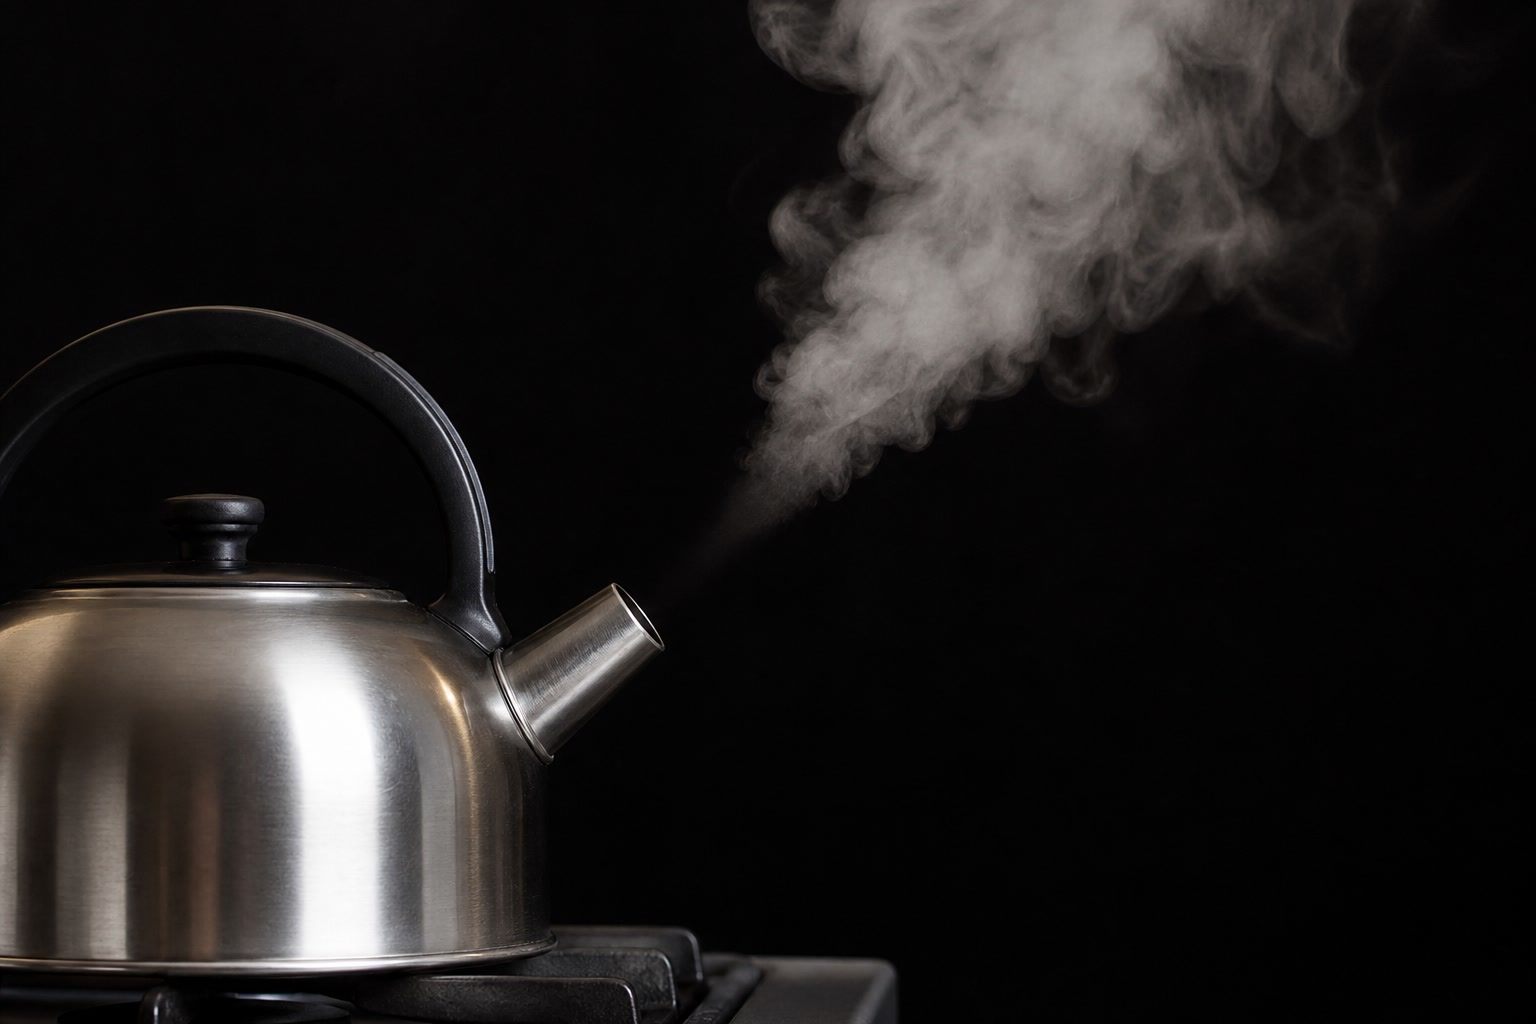
\includegraphics[width=0.55\linewidth]{images/book1/ai/g2-ice-water-steam-kettle.jpg}

{\small O segredo da chaleira: logo acima do bico, um pequeno espaço \emph{transparente} em que a água é um gás invisível --- só mais acima ela se \omterm{def:g2:ice-water-steam:evapcond}{condensa} na pluma branca que conseguimos ver.}
\end{omfigure}

\section{Mudar de estado}

\begin{definition}[Derreter e congelar]\label{def:g2:ice-water-steam:meltfreeze}
Quando o calor transforma o gelo sólido em água líquida, o gelo
\emph{derrete}\index{derreter}. Quando o frio forte transforma a água
líquida em sólido, a água \emph{congela}\index{congelar}. Derreter e
congelar são portas opostas entre os mesmos dois estados: o calor
empurra para um lado, o frio empurra para o outro.
\end{definition}

\begin{definition}[Evaporar e condensar]\label{def:g2:ice-water-steam:evapcond}
Quando o calor faz a água líquida voar para o ar como gás, a água
\emph{evapora}\index{evaporar} --- a poça encolhe, a roupa seca.
Quando o vapor de água encosta em alguma coisa fria e volta a virar
gotinhas de líquido, ele \emph{condensa}\index{condensar} --- o
embaçado na janela fria, a névoa no espelho do banheiro. De novo duas
portas opostas: o calor manda a água para o estado gasoso, o frio a
chama de volta para o líquido.
\end{definition}

\begin{omfigure}
\begin{tikzpicture}[scale=0.85]
  \node[font=\small, draw, thick, omDef, minimum width=1.9cm,
    minimum height=0.85cm] (ice) at (0.8,0) {sólido};
  \node[font=\small, draw, thick, omDef, minimum width=1.9cm,
    minimum height=0.85cm] (water) at (5.3,0) {líquido};
  \node[font=\small, draw, thick, omDef, minimum width=1.9cm,
    minimum height=0.85cm] (steam) at (9.8,0) {gasoso};
  \draw[-Stealth, very thick, omThm] (1.85,0.28) -- (4.25,0.28);
  \node[above, font=\small, omThm] at (3.05,0.42) {calor: derrete};
  \draw[-Stealth, very thick, omDef] (4.25,-0.28) -- (1.85,-0.28);
  \node[below, font=\small, omDef] at (3.05,-0.42) {frio: congela};
  \draw[-Stealth, very thick, omThm] (6.35,0.28) -- (8.75,0.28);
  \node[above, font=\small, omThm] at (7.55,0.42) {calor: evapora};
  \draw[-Stealth, very thick, omDef] (8.75,-0.28) -- (6.35,-0.28);
  \node[below, font=\small, omDef] at (7.55,-0.42) {frio: condensa};
\end{tikzpicture}

{\small As mudanças de estado: o calor sempre empurra para a direita,
o frio sempre empurra de volta para a esquerda.}
\end{omfigure}

\begin{example}[Experimente: pegue a água invisível]\label{ex:g2:ice-water-steam:catch}
Pegue uma lata ou um copo recém-tirado da geladeira, seque bem a
parte de fora com um pano e ponha sobre a mesa. Espere enquanto conta
até $100$. A parte de fora fica embaçada e depois molhada --- surgem
gotas do nada! Elas não estão vazando através do vidro: o vapor de
água invisível do ar do cômodo encostou na parede fria e se
condensou. Você acabou de pegar o gás invisível.
\end{example}

\begin{example}[Nuvens de respiração]\label{ex:g2:ice-water-steam:breath}
A sua respiração sempre carrega vapor de água invisível. Num dia
quente ele continua invisível. Numa manhã gelada, o ar frio da rua o
\omterm{def:g2:ice-water-steam:evapcond}{condensa} na hora numa nuvenzinha na frente da sua boca --- e o mesmo
acontece numa janela fria quando você assopra nela para desenhar com
o dedo.
\end{example}

\begin{remark}[Vapor e fogão: cuidado]\label{rem:g2:ice-water-steam:safety}
O vapor de água acima de uma panela fervendo queima --- ele é mais
quente do que a própria água parece. Nunca ponha a mão dentro da
pluma, e levante as tampas para o lado contrário ao do seu rosto, com
um adulto por perto. Sempre que houver um fogão envolvido, as
mudanças de estado são para ver, não para tocar.
\end{remark}

\section{A mesma água, dando voltas}

\begin{example}[A poça que encolhe]\label{ex:g2:ice-water-steam:puddle}
Depois da chuva, uma poça brilha no pátio. À tarde ela já encolheu;
amanhã terá sumido. Ninguém a bebeu e ela não vazou pelo asfalto: o
calor do Sol a fez \omterm{def:g2:ice-water-steam:evapcond}{evaporar}, gota a gota, para o ar. Desenhe um
contorno de giz em volta de uma poça de manhã e confira depois do
almoço: a água recuou para dentro do seu contorno.
\end{example}

\begin{example}[Do mar até a chuva]\label{ex:g2:ice-water-steam:cycle}
O que \omterm{def:g2:ice-water-steam:evapcond}{evapora} tem de se \omterm{def:g2:ice-water-steam:evapcond}{condensar} em algum lugar. A água sobe dos
mares e das poças, invisível; lá no alto do céu, onde o ar é frio,
ela se \omterm{def:g2:ice-water-steam:evapcond}{condensa} nas gotinhas que formam as nuvens; as gotinhas se
juntam, ficam pesadas e caem --- chuva! A chuva enche as poças e os
mares, e a viagem de ida e volta recomeça. A água do seu copo já fez
essa viagem mais vezes do que qualquer pessoa consegue contar.
\end{example}

\section{Exercícios}

\begin{exercise}[$\star$]\label{exo:g2:ice-water-steam:1}
Em que estado da matéria está cada um destes --- sólido, líquido ou
gasoso: um pingente de gelo; \ o mar; \ a água invisível logo acima
do bico da chaleira; \ a geada no capim; \ a chuva?
\end{exercise}

\begin{exercise}[$\star$]\label{exo:g2:ice-water-steam:2}
Diga o nome da mudança de estado: um boneco de neve encolhendo no
sol; \ uma poça sumindo; \ o embaçado aparecendo no espelho do
banheiro; \ um lago ficando duro no inverno.
\end{exercise}

\begin{exercise}[$\star$]\label{exo:g2:ice-water-steam:3}
No desenho das mudanças de estado, para que lado o calor sempre
empurra: para o sólido ou para o gás? E o frio?
\end{exercise}

\begin{exercise}[$\star$]\label{exo:g2:ice-water-steam:4}
As gotas na lata gelada do \cref{ex:g2:ice-water-steam:catch} ---
elas vazaram através do vidro? De onde elas vieram?
\end{exercise}

\begin{exercise}[$\star$]\label{exo:g2:ice-water-steam:5}
Por que você enxerga a sua respiração numa manhã gelada e não num dia
quente? Use as palavras da \cref{def:g2:ice-water-steam:evapcond}.
\end{exercise}

\begin{exercise}[$\star$]\label{exo:g2:ice-water-steam:6}
Roupa molhada seca mais depressa no sol do que na \omterm{def:g1:light-and-shadows:shadow}{sombra}. Qual
mudança de estado está trabalhando, e o que o Sol acrescenta para
acelerá-la?
\end{exercise}

\begin{exercise}[$\star$]\label{exo:g2:ice-water-steam:7}
Por que a pluma acima de uma panela fervendo é perigosa, e qual é a
regra de segurança da \cref{rem:g2:ice-water-steam:safety}?
\end{exercise}

\begin{exercise}[$\star$]\label{exo:g2:ice-water-steam:8}
Conte a viagem de ida e volta de uma gota de chuva: comece no mar,
termine de volta no mar e use as palavras \omterm{def:g2:ice-water-steam:evapcond}{evaporar} e \omterm{def:g2:ice-water-steam:evapcond}{condensar} no
caminho.
\end{exercise}

\begin{exercise}[$\star\star$]\label{exo:g2:ice-water-steam:9}
No bico da chaleira há um espaço transparente, e só acima dele
começa a pluma branca. O que há nesse espaço transparente? O que isso
mostra sobre a água no estado gasoso?
\end{exercise}

\begin{exercise}[$\star\star$]\label{exo:g2:ice-water-steam:10}
Nino deixa um copo de água no parapeito da janela durante uma semana;
o nível baixa dia após dia, embora ninguém beba dela. O gato dele é
acusado. Defenda o gato: explique o que aconteceu de verdade e
invente um jeito de mostrar que a água vai embora \emph{para o ar}, e
não para dentro do gato.
\end{exercise}
